%%%%%%%%%%%%%%%%%%%%%%%%%%%%%%%%%%%%%%%%%%%%%%%%%%%%%%%%%%%%%%%%%%%
%                                                                 %
%                            CHAPTER FOUR                         %
%                                                                 %
%%%%%%%%%%%%%%%%%%%%%%%%%%%%%%%%%%%%%%%%%%%%%%%%%%%%%%%%%%%%%%%%%%%

\chapter{SCALABLE PARALLEL MESH ADAPTATION}
\label{chap:parallel}
\blfootnote{
Portions of this chapter previously appeared as:
D.~A. Ibanez, E.~S. Seol, C.~W. Smith, and M.~S. Shephard, ``Pumi: Parallel
  unstructured mesh infrastructure,'' \emph{ACM Trans. Math. Softw.}, vol.~42,
  no.~3, pp. 17:1--17:28, May 2016.
}\nocite{ibanez2016pumi}
\blfootnote{
Portions of this chapter previously appeared as:
D.~Ibanez, I.~Dunn, and M.~S. Shephard, ``Hybrid mpi-thread parallelization of
  adaptive mesh operations,'' \emph{Parallel Comput.}, vol.~52, pp. 133 -- 143,
  Jan. 2016.
}\nocite{ibanez2016hybrid}
\blfootnote{
Portions of this chapter previously appeared as:
D.~Ibanez and M.~Shephard, ``Mesh adaptation for moving objects on shared
  memory hardware,'' in \emph{Proc. 25th Int. Meshing Roundtable}.\hskip 1em
  plus 0.5em minus 0.4em\relax Washington, DC: Elsevier, Sep. 16--29, 2016.
}\nocite{ibanez2016mesh}

\section{Defining Scalability}
\label{sec:scalable}

It is important to first define scalability in the context of
parallel computers.
First, we define a single scalar $N$ describing the problem size.
For mesh-based simulations, the number of mesh elements
is a good approximate measure of problem size.
Then we consider any operation which would take $O(N)$ time to execute
on a single processor such as the reference computer
in Section \ref{sec:ref_comp}, and analyze the runtime bound
of this operation when it is parallelized using $P$ cooperating processes.
When this the parallel runtime is $O(N/P)$, we say the operation
has perfect linear scaling.
Linear scaling typically only occurs when the processes do not have to coordinate,
and coordination usually adds a factor $\log(P)$ to the runtime,
meaning that the operation takes $O((N/P)\log(P))$ time in parallel.

Notice that we are considering a single operation which takes $O(N)$
time in serial.
For example, a Recursive Inertial Bisection partitioning method is a
divide-and-conquer algorithm which uses $O(\log(P))$ steps, each
taking $O(N)$ time, to assign $N$ items to $P$ partitions
for a total serial runtime which is $O(N\log(P))$
(analogous to an incomplete sorting algorithm)
\cite{simon1991partitioning}.
If the items are already well partitioned amongst $P$ processes
and we run a parallel version of this procedure to adjust the
partitioning, each $O(N)$ step becomes $O((N/P)\log(P))$
and the whole operation can be expected to take $O((N/P)\log^2(P))$.

Next, we define parallel runtime bounds which are considered non-scalable.
The simplest example is one where an $O(N)$ serial operation becomes
an $O(N)$ parallel operation, i.e. there is asymptotically no scaling.
Although trivial, an alarming number of parallel programs in production
use exhibit this degree of scaling for key parallel operations
(for example, partitioning is done is serial prior to a parallel simulation).
Because non-scalable operations may not consume a large percentage
of runtime at low degrees of parallelism,
these systems can show good parallel speedups up to a certain degrees of parallelism,
but ultimately run into difficulties for large $P$ ($10^6$).
The second example is an operation which has $O(P)$ runtime in parallel.
Once again, may systems in production use today suffer from such
trivial non-scalability.
For example, it is natural when organizing communications for each process to create
an array of size $P$ with information about what is being sent to each
other process (or worse, to actually send data to every other cooperating process).
The continued use of $O(P)$ algorithms is a significant obstacle to
increasing the degree of shared memory parallelism in leadership-class supercomputers.
The issue is made worse by the fact that until fairly recently,
MPI (see Section \ref{sec:def_mpi}) itself would either use
or encourage the use of such algorithms \cite{balaji2009mpi}.
Section \ref{sec:paraops} describes how to use modern MPI
to avoid non-scalable operations during communication.

All the above considerations have analogues for the case of shared-memory programming,
in which case one can exchange the number of parallel processes $P$ for a number
of parallel threads $T$.
In the case of shared memory only, there are fewer communication concerns because
all threads may access all data directly.
Although there are Non-Uniform Memory Access (NUMA) costs incurred if threads do
not organize their data to minimize sharing, these costs are much smaller than
the cost of network communication.

\section{Parallel Operations}
\label{sec:paraops}

In this section we introduce a set of key collective parallel operations
used to write parallel programs.
All of these are scalable operations as described in Section \ref{sec:scalable}.
As such, a good approach to designing scalable programs is to use
only these operations for parallelism.

\subsection{Map}
\label{sec:map}

This is the most basic parallel operation, and is included to
place our definitions in the context of the map-reduce programming model which
has gained popularity in processing Internet data sets \cite{dean2008mapreduce}.
The simplest definition of a map operation takes in an array $\mathbf{a}=\{a_0,a_1,a_2,...a_N\}$
and a unary operator $f$ and returns an array
$\mathbf{b}=\{f(a_0), f(a_1), f(a_2),...,f(a_N)\}$.

We generalize it to the idea of running $N$ independent
operations in parallel with no need for coordination.
The shared memory implementation of a map operation is the \texttt{parallel\_for}
concept introduced in Section \ref{sec:openmp}.
The need for these operations to be independent often forces the result to exist
as one or more arrays of $N$ result values.
The distributed memory implementation is anything inside a normal MPI program.
Since MPI processes always execute in parallel, anytime all processes perform
the same operation without coordination (message passing), it can be interpreted
as an implicit map operation.
This illustrates an important distinction between MPI programming and shared
memory programming: MPI is parallel by default, while shared memory programming
environments like OpenMP and CUDA are serial by default and parallelism
must be explicitly requested per operation.

The map operation is the prime example of an operation which scales
perfectly.
Assuming the operator $f$ requires $O(1)$ time, a serial execution
requires $O(N)$ time and a parallel operation over $P$ processes
and $T$ threads takes $O(N/(PT))$ time.

\subsection{Reduce}
\label{sec:reduce}

A reduction operation takes as input an array
$\mathbf{a}=\{a_0,a_1,a_2,...,a_N\}$ of scalar values and
a binary operator $\otimes$, and returns a single scalar result.
The result is related to the array entries via a binary expression tree,
and in order to allow flexibility of implementation, any valid binary
tree may be used.
Figure \ref{fig:reduce} shows two valid binaries trees an implementation
may use to reduce an array of five entries.
The value of a leaf node in this tree is the value of a unique array entry,
and the value of the non-leaf nodes is the result of applying
the binary operator to the values of its two child nodes.
The value of the root of the tree is the overall reduction result.

The left tree in Figure \ref{fig:reduce} illustrates the typical
serial reduction process of maintaining an accumulator value and
adding each consecutive array entry to it.
The right tree in Figure \ref{fig:reduce} illustrates the most theoretically
scalable implementation, i.e. a balanced tree.
Assuming we have as many parallel processes as we have array entries,
each of the $\lceil\log(N)\rceil$ layers of the balanced tree
can be evaluated simultaneously and the
runtime to evaluate the reduction is $O(\log(N))$ for arrays of size $N$.
However, the balanced tree requires $O(N)$ memory for the intermediate
result at one layer, while the serial tree can be evaluated with
a single accumulator ($O(1)$ memory).
The memory requirement is one reason why the serial tree is chosen
in cases when no parallelism is available.

If we have fewer parallel processes than array entries, we can use a hybrid mix
of the two trees in Figure \ref{fig:reduce}, where each processor
uses a serial tree to reduce $O(N/P)$ values in $O(N/P)$ time, and
then each process' local results are reduced using a balanced tree
in $O(\log(P))$ time resulting in an $O((N/P)+\log(P))$ runtime.

The binary operators used most often in Omega\_h reductions
are the sum, minimum, and maximum of the two inputs.
Notice that the ability of implementations to choose any tree
is a problem when the operator $\otimes$ is not commutative
(the result depends on the tree structure),
as is the case with typical computer implementations of floating-point summation.
Section \ref{sec:repro_sum} will describe a technique for dealing
with this issue.

\begin{figure}
\begin{center}
\includegraphics[width=0.7\textwidth]{reduce.png}
\caption{Two possible binary trees used for reduction}
\label{fig:reduce}
\end{center}
\end{figure}

The shared memory implementation of reductions is in our case
provided by the Kokkos library's \texttt{Kokkos::parallel\_reduce}
function \cite{edwards2013kokkos}.
The distributed memory implementation (which accepts a single value
per process) is provided by MPI's \texttt{MPI\_Reduce} and \texttt{MPI\_Allreduce}
functions (the later makes the result available to all processes, which is
often desired).
Combining these gives a reduction that can be expected to
complete in $O((N/(PT))+\log(PT))$ time.

\subsection{Scan}
\label{sec:scan}

Scan operations are key to scalable parallel programming, especially when using
arrays for storage.
Given an input array $\mathbf{a}=\{a_0, a_1, a_2, ..., a_N\}$ and a binary operator
$\otimes$, an inclusive scan returns an array $\mathbf{b}=\{b_0, b_1, b_2, ..., b_N\}$
where each $b_i=\text{reduce}(\{a_0, a_1, a_2, ..., a_i\}, \otimes)$, i.e. the
$i$-th output value is the result of reducing the first $i$ input values.
An exclusive scan differs in that the $i$-th output value is the reduction
of the first $(i-1)$ values only (meaning the first output value must be defined separately).
A scan with $(\otimes)=(+)$ is often referred to as a prefix sum.

Intuitively, a scan operation may be implemented with help from the intermediate
values of a reduction tree.
For example, the intermediate values in the serial tree (Figure \ref{fig:reduce}(left))
are exactly the output values for scanning, meaning a scan takes $O(N)$ time in serial.
Parallel scanning is a bit more complex and requires essentially traversing a
balanced tree twice (Figure \ref{fig:reduce}(right)), which still gives
it a time complexity of $O(\log(N))$ assuming as many processors as input values.

We use the \texttt{Kokkos::parallel\_scan} function to provide the shared
memory implementation of scans, and the \texttt{MPI\_Exscan} function
to provide the distributed memory implementation, which accepts one
value per process.

The utility of exclusive scans is in generating offsets for sub-groups of items in
a global collection based on the size of each subgroup.
For example, given the number of mesh elements per part, the \texttt{MPI\_Exscan}
takes $O(\log(P))$ time to returns offsets which can be used to establish a global
numbering of mesh elements without further communication.
Likewise, given the number of edges adjacent to each mesh vertex, a
\texttt{Kokkos::parallel\_scan} takes $O((N/T)\log(T))$ to produce offsets
for all vertices that allow the construction of compressed-row
storage for the vertex-to-edge adjacency (see Section \ref{sec:adj_arr}).

\subsection{Sort}
\label{sec:sort}

Although we do not yet require a full distributed memory sorting algorithm
in our work, we do have uses for sorting at the shared memory level
(see Section \ref{sec:reorder}), so we include this as a key parallel operation.
In Omega\_h, we use a slightly unusual definition of sorting:
given an array $\mathbf{k}=\{k_0,k_1,k_2,...,k_N\}$ of keys and
a strict weak ordering $(\prec)$ \cite{roberts2009applied},
return a permutation array
$\mathbf{p}=\{i_0,i_1,i_2,...,i_N\}$ which indicates
a sorted order for $\mathbf{k}$, meaning that ($k_{i_j} \prec k_{i_{j+1}}$).
We use this definition so that the permutation array can be re-used
to sort multiple other arrays that are associated with the array of keys.
We also require that the algorithm be stable (keys which are ``equal"
in the ordering $(\prec)$ retain the same relative order) for
determinism reasons.
This is especially important when other arrays are being sorted
using the permutation array.

Implementing a parallel sorting algorithm is considerably more
challenging than implementing scans and reductions.
At the time of this writing, Kokkos does not offer a highly general
sorting capability.
Instead, Omega\_h relies on the Thrust library to provide sorting functionality
on GPUs \cite{bell2011thrust}.
There several algorithms for sorting on GPUs \cite{satish2009designing},
ranging in complexity up to $O((N/T)\log^2(N))$, which we still consider
scalable.
On manycore CPUs, we use a parallel merge sort implementation provided
by researchers at Intel \cite{robinson2014parallel}.

\subsection{Exchange}
\label{sec:exch}

We use the term exchange to refer to the distributed memory operation
in which each process has a set of messages to send, each message
having a unique destination process, and these messages are exchanged
such that each process receives all the messages addressed to it
during the operation.
The difficult part of implementing an exchange is determining, for
a given destination process, the full set of messages addressed to it.
Hoefler, Siebert, and Lumsdaine \cite{hoefler2010scalable} describe
a communication-optimal algorithm for conducting a ``sparse dynamic exchange".
They define a sparse exchange as one in which the number of messages
sent from or received by any single process is $O(\log(P))$.
This is important, because if a process tries to send $O(P)$ messages
then it is impossible to execute the exchange in a scalable way.
They define a dynamic exchange as one in which the set of messages
a process must receive is unknown to that process at first, hence
the difficulty described above.

Many codes in use today solve this problem by using a variant
of the ``personalized consensus" algorithm in \cite{hoefler2010scalable},
reproduced here as Algorithm \ref{alg:pcx}.
By relying on a table (array) of size $P$, this algorithm is
non-scalable.
A scalable solution is the ``non-blocking consensus" algorithm
in \cite{hoefler2010scalable}, seen here as Algorithm \ref{alg:nbx}.
This algorithm uses synchronous sends, meaning that when a message
is received at its destination, a confirmation is returned to the
sender.
Once a process receives confirmation that all its outgoing messages
reached their destinations, it enters the non-blocking barrier.
This barrier can execute concurrently with other message traffic,
and once all processes enter it, it will signal its completion
to all processes.
Upon detecting completion, a process can be sure that all messages
in flight have been received, thus it is safe to stop waiting for
incoming messages.
The barrier must be non-blocking because in order to make progress,
processes must be able to continue receiving incoming messages
until the time of overall completion.
Knowing the communication is sparse, this algorithm runs in $O(\log(P))$
time \cite{hoefler2010scalable}.

\begin{algorithm}
\caption{Personalized Consensus \cite{hoefler2010scalable}}
\label{alg:pcx}
\SetKwInOut{Input}{input}\SetKwInOut{Output}{output}
\Input{List $S$ of destinations and data}
\Output{List $R$ of received data and sources}
allocate local table with $P$ entries, initialize all entries to `0'\;
\ForEach{$i \in S$}{
  set row target($i$) in local table to `1'\;
}
$g=$ global sum of my table row\;
\ForEach{$i \in S$}{
  start nonblocking sends to dest($i$)\;
}
\For{\algt round from $1$ to $g$}{
  msg $=$ blocking probe for incoming message\;
  allocate buffer, receive message, add buffer to $R$\;
}
\end{algorithm}

\begin{algorithm}
\caption{Non-Blocking Consensus \cite{hoefler2010scalable}}
\label{alg:nbx}
\SetKwInOut{Input}{input}\SetKwInOut{Output}{output}
\Input{List $S$ of destinations and data}
\Output{List $R$ of received data and sources}
done$=$false\;
barrier\_active$=$false\;
\ForEach{$i \in S$}{
  start nonblocking synchronous send to process dest($i$)\;
}
\While{\algt not (done)}{
  msg = nonblocking probe for incoming message\;
  \If{\algt msg exists}{
    allocate buffer, receive message, add buffer to $R$\;
  }
  \eIf{\algt barrier\_active}{
    comp $=$ test barrier for completion\;
    \lIf{comp}{done$=$true}
  }{
    \If{\algt all sends are finished}{
      start nonblocking barrier\;
      barrier\_active$=$true\;
    }
  }
}
\end{algorithm}

Section \ref{sec:pcu_phased} describes how PUMI's communication
library, PCU, implements Algorithm \ref{alg:nbx}.
This implementation goes beyond MPI because it is designed to
allow communication between operating system threads instead
of just processes.

As of the MPI 3.0 standard, however, it is no longer necessary to
program one's own exchange algorithm, as it can be accomplished
by combining two key MPI systems:
scalable process topology (graph communicators) \cite{hoefler2011scalable},
and neighborhood collectives \cite{hoefler2012optimization}.
This is the approach taken for distributed memory exchanges
in Omega\_h.

MPI's neighborhood collective functions perform non-dynamic
exchanges, meaning that they must be informed of the incoming
as well as outgoing messages.
This is semantically the same as performing a series of single-message
sends and receives, but comes with a few benefits.
First, MPI's understanding that the messages are all to be
sent at once enables it to perform certain optimizations.
Second, the interface specifies that the data for all
outgoing messages is to be packed in a single array
(with data going to the same destination being contiguous).
This is good for integrating MPI with shared-memory
code, because the shared-memory code may efficiently prepare
the outgoing data array and may efficiently process the incoming
data array, thus minimizing the amount of work done by MPI
(which is not guaranteed to use shared-memory parallelism to
accelerate its work).
Unfortunately, the neighborhood collective exchange functions
have the name prefix \texttt{MPI\_Neighbor\_alltoall}, where
\texttt{alltoall} is too reminiscent of the non-scalable practice
of transmitting $O(P)$ messages from one processor.

The remaining problem of determining messages to receive can
be delegated to MPI's scalable process topology description
via the function \texttt{MPI\_Dist\_graph\_create}.
First, note that the above process is a graph theoretical problem
of determining incoming graph edges to a graph node when each
graph node knows only its outgoing edges.
\texttt{MPI\_Dist\_graph\_create} allows each process to specify
any subset of the edges in the communication graph, and assumes
responsibility for informing each process of all its incoming
and outgoing edges.
This is a more general and difficult problem than the one described
above, and we restrict our use of this function to having each
process specify all its outgoing edges.
Given this restriction, we assume it executes in $O(\log(P))$ time.

Note that the exchange operation does not have a clear shared-memory equivalent
in the context of Omega\_h,
because accessing shared memory directly is preferred over sending
explicit messages amongst threads.

\section{PCU: Scalable Inter-Thread Communication}
\label{sec:pcu}

PCU is a library that provides a parallel programming model including
parallel control functions.
Its two major functionalities are message passing that allows parallel tasks to
coordinate and thread management that extends the MPI programming model
into a hybrid MPI/thread system.

The foundation of PCU is its point-to-point message passing routines where
non-blocking synchronous message passing primitives are defined. There are
two versions, one of which is a direct interface to MPI, and the second supports
message passing between threads \cite{ibanez2016hybrid}. The two versions
are interchangeable, and PCU can change which set of them is being used at
run-time without affecting the rest of software components.

Building on the point-to-point primitives, PCU has an extensible framework for
collective operations such as reduction, broadcast, scan, and barrier.
Any collective whose communication pattern can be encoded as some kind of tree
is supported, and the most common ones come built-in to PCU.
These collectives are directly available to users.

Using both collectives and point-to-point communication, PCU provides a flexible
user interfaces similar to MPI 3.0's \texttt{MPI\_Neighbor\_alltoallw}.
The first phase
allows tasks to construct messages to multiple neighbors
at once and then send them.
The second phase ensures that neighbors
receive all the messages they have been sent.
This ``phased" communication algorithm is
conceptually the same as Algorithm \ref{alg:nbx}.

Finally, PCU has a system for creating a pool of threads within each process and
assigning them ranks the way MPI does to processes.
Users can call this API to enter a hybrid MPI+threads mode in which all the
communication APIs (point-to-point, collective, and phased) work between
threads.
These capabilities support PUMI's overall hybrid MPI+thread operation.

\subsection{Messaging Primitives in PCU}
\label{sec:pcu_p2p}

The main unusual design choice of PCU compared to
other hybrid programming systems is
its focus on inter-thread message passing.
Since we must rebuild some of the high-level message
passing capabilities, we identify a set of primitive
operations as described by the MPI standard \cite{gropp1996mpi}
which are sufficient for our applications:

\begin{enumerate}
\item Non-blocking synchronous send
\item Non-blocking send request completion test
\item Non-blocking probe
\item Blocking receive
\end{enumerate}

These conceptual message-passing primitives are independent
of their particular implementation.
Note that because we require the send operation to be synchronous,
it will complete if and only if the message is completely received at its
destination.

All the remaining algorithms rely only on these guaranteed properties
of the message passing primitives.
To develop inter-thread message passing, we implement inter-thread
message passing passing primitives.
These are currently based on calling thread-safe MPI versions of the
same primitives, but an area of future work involves implementing
more efficient primitives.

In order to use MPI itself to pass messages between threads, we require
that the implementation correctly handle self-sends.
Then, we need to encode the source and destination thread IDs into the message
metadata such that messages can be multiplexed out of a single process
and demultiplexed at their destination process.
The encoding of thread IDs makes use of the standard \texttt{MPI\_TAG} metadata
integer, which is typically a 32-bit signed integer.
We use 10 bits of this integer to encode each of the local IDs for the
source and destination threads.
This encoding of source and destination means that threads must inspect
messages with more sophisticated checking of the tag than
\texttt{MPI\_Recv}
offers, since messages arriving at the same process may be destined
for different threads within that process.
We use \texttt{MPI\_Iprobe} to inspect the tag before using
\texttt{MPI\_Recv} to commit to being the receiver.
This combined probe and conditional receive procedure is specified
in Algorithm \ref{alg:receive}.

\begin{algorithm}
\LinesNumbered
\SetKwInOut{Input}{input}\SetKwInOut{Output}{output}
\Input{pattern $P$}
\Output{received message metadata $M$ and data $b$, or null}
let message $M \gets$ non-blocking probe\;
\If{\algt $M$ is null (there is no message)}{
  \Return null\;
}
\If{\algt metadata of $M$ does not match $P$}{
  \Return null\;
}
allocate buffer $b$ per metadata of $M$\;
blocking receive $M$ into $b$\;
\Return $(M,b)$\;
\caption{Non-blocking pattern-match receive}
\label{alg:receive}
\end{algorithm}

\subsection{Simple Collectives in PCU}
\label{sec:pcu_coll}

Collective operations are a necessary staple of
distributed-memory high-performance computing.
Operations such as parallel reduction, broadcast, and other collectives
are key to coordinating threads \cite{pjevsivac2007performance}.
More details on these collective algorithms and tradeoffs in their
implementation can be found in \cite{thakur2003improving}.
Non-blocking collectives are more advanced implementations which
are typically used to overlap communication and computation.
By using them, PCU benefits from this overlap.
Furthermore, in Section \ref{sec:pcu_phased}, we use Algorithm \ref{alg:nbx}
for which a non-blocking implementation is necessary.

Since collectives are used by nearly all applications,
we place a focus on developing built-in
multithreaded collective operations based on the
inter-thread message passing primitives.

We consider three fundamental collective operations:
broadcast, reduce, and scan.
Other operations such as exclusive scan and all-reduce
can be built from the first three.
These operations were selected as the minimal subset
of collectives needed for our unstructured mesh operations.

These three collectives share many common features:
they use $O(\log n)$ steps for $n$ threads,
and at each step each thread is either idle, sending one
message, or receiving one message.
These shared characteristics make it easier to implement
all the collectives in a general framework which abstracts
away their differences, starting with the specific communication
pattern used.
A thread only needs to know which of the three actions to perform at each
step and with which thread it is communicating, if any.
This combined information is referred to as the communication pattern.

The second abstraction we can make is that of a merge operator, which is
essentially the MPI reduction operator
(e.g. \texttt{MPI\_SUM} or \texttt{MPI\_MAX}).
The merge operator modifies the local data based on incoming data.
For example, an reduction sum adds incoming values to local values.
We do not refer to it as the reduction operator because it is used
in all cases, including broadcast.
As an interesting corner case, the merge operator for broadcast simply
assigns the incoming value as the local value.

Following good software design, the communication pattern,
merge operator, and data are each specified separately
and are orthogonal from one another.
This follows the example of interfaces such as \texttt{MPI\_Reduce}.

With these abstract components specified, we can execute a collective
operation
using the non-blocking point-to-point message passing primitives
developed in Section \ref{sec:pcu_p2p}.
Although the simplicity of collectives would allow blocking primitives
to be used, using non-blocking primitives gives us a great benefit:
we obtain a non-blocking collective operation.
Such operations were implemented by Hoefler and Lumsdaine outside MPI
\cite{hoefler2007implementation}
and their subsequent proposal to make them part of the MPI standard
\cite{hoefler2007case} was accepted.
Our work implements hybrid threaded versions of such collectives.

Users of this system initiate a collective operation, and can interleave
computation with communication progress queries.
Communication progress consists of checking for incoming messages in the current
step and proceeding to the next step when they are received.

Non-blocking collectives are useful from the perspective of
of hiding latency, but they prove to be indispensable to
Algorithm \ref{alg:nbx}.

As a detailed example of how our non-blocking collectives work,
Algorithms \ref{alg:start_reduce} and \ref{alg:progress_reduce}
show the functions that would begin and advance a non-blocking
reduction, respectively.
In these algorithms we use $\wedge$ to denote a bitwise and
operation and $\oplus$ to denote a bitwise exclusive or operation.
The operator $\otimes$ continues to represent the binary reduction,
e.g. summation.
Several helper functions were inlined for brevity, hence there
is some repetition.
For example, the termination condition on line 4 of Algorithm
\ref{alg:start_reduce} and lines 1 and 14 of Algorithm \ref{alg:progress_reduce}.
This condition is one of the aspects which varies depending on
which type of collective is being executed (broadcasts and scans
have different logic here).
We implement a balanced binary tree (similar to Figure \ref{fig:reduce}(right))
based on the binary digits of the thread ID (rank).

\begin{algorithm}
  \SetKwInOut{Input}{input}\SetKwInOut{Output}{output}
  \Input{local data $d_l$}
  peers $\gets$ total thread count\;
  rank $\gets$ local thread rank $\in[0,$peers$-1]$\;
  bit $\gets 1$\;
  \If{\algt ((rank$=0$) and (bit$\geq$peers)) or \\
      ((rank$\neq0$) and (((bit$/2$)$\wedge$rank)$\neq0$))}{
    \Return\;
  }
  \If{\algt rank$\oplus$bit$<$peers}{
    \If{\algt bit$\wedge$rank$\neq0$}{
      request $\gets$ send $d_l$ to (rank$\oplus$bit)\;
    }
  }
  \Return{\algt state as (bit,request)}
  \caption{Starting a non-blocking reduction}
  \label{alg:start_reduce}
\end{algorithm}

\begin{algorithm}
  \SetKwInOut{Input}{input}\SetKwInOut{Output}{output}
  \Input{access to local data $d_l$}
  \Input{access to state tuple (bit,request)}
  \If{\algt((rank$=0$) and (bit$\geq$peers)) or \\
      ((rank$\neq 0$) and (((bit$/2$)$\wedge$rank)$\neq0$))}{
    \Return{\algt false}\;
  }
  step\_done $\gets$ false\;
  \lIf{\algt rank$\oplus$bit$\geq$peers}{step\_done $\gets$ true}
  \Else{
    \If{\algt bit$\wedge$rank$\neq0$}{
      \lIf{\algt request is done}{step\_done $\gets$ true}
    }\Else{
      \If{\algt received message from (rank$\oplus$bit) with data $d_r$}{
        $d_l \gets d_l \otimes d_r$\;
        step\_done $\gets$ true\;
      }
    }
  }
  bit $\gets 2\cdot$bit\;
  \If{\algt ((rank$=0$) and (bit$\geq$peers)) or \\
      ((rank$\neq 0$) and (((bit$/2$)$\wedge$rank)$\neq0$))}{
    \Return{\algt false}\;
  }
  \If{\algt rank$\oplus$bit$<$peers}{
    \If{\algt bit$\wedge$rank$\neq0$}{
      request $\gets$ send $d_l$ to (rank$\oplus$bit)\;
    }
  }
  \Return{\algt true}
  \caption{Progress a non-blocking reduction}
  \label{alg:progress_reduce}
\end{algorithm}

\subsection{Non-blocking Consensus in PCU}
\label{sec:pcu_phased}

A common problem that arises when dealing with parallel graphs,
and similar structures, such as the adjacency relations of unstructured
meshes, has to do with transporting graph, or mesh entities, from
one thread to another
due to changes in the graph or to other operations which affect
load balance.
Such transportation is specified in a one-sided,
push-driven manner, which means that each thread knows which
entities it should send to which other threads, but does
not know what it will be receiving.

Without {\it a priori} knowledge of the extent of information to be
received, it is difficult to determine when to stop receiving
information.
A thread can perform a continuous loop which receives messages,
but we must determine when to terminate that loop.

This problem has been solved previously in a slightly less efficient
manner \cite{ovcharenko2012neighborhood}, and is an important special case
of the general termination detection problem.
PCU implements an optimal solution based on Algorithm \ref{alg:nbx}
described in Section \ref{sec:exch}.
Note that Algorithm \ref{alg:nbx} overlaps all incoming message processing
with all outgoing message wait operations, so the potential for latency
hiding is maximized.

When implementing phased message passing, we also optimize performance
by buffering small messages.
Users see an interface which allows sending small amounts of data to
any destination.
The user interface of phased communication allows us to pack
all data traveling between the same pair of threads into a single message.
This is done prior to executing Algorithm \ref{alg:nbx}, which expects
that the number of messages sent $|S|$ is equal to the number of unique
destinations and the number of messages received $|R|$ is equal to the number
of unique sources.

This relation of message counts to communication neighbors (sources and
destinations) is quite useful in the process of determining runtime bounds.
This is because, due to mesh partitioning, each thread should have a small
and constant number of neighbors, with 40 being a maximum value among
several meshes studied \cite{zhou2010petascale}.

We have shown previously that buffering small messages can greatly improve performance
due to the latency cost $\alpha$ and MPI's own management overhead per message,
especially for applications
with a tendency to send very small messages between the same pair of threads
\cite{ovcharenko2012neighborhood}.
In the case of multiple threads per process, buffering also reduces
the number of calls to \texttt{MPI\_Send} and \texttt{MPI\_Recv}, which reduces
contention for the MPI library between the threads in that process.
When these calls are protected by a lock, avoiding contention is important
\cite{mavriplis2002parallel}.

\section{Remote Copies and Owners}
\label{sec:remotes}

For distributed memory parallelism, we are required to separate our
data amongst multiple memory spaces.
In order to find a piece of data across an entire distributed memory
machine, one needs to pieces of information: which of the
memory spaces it is in, and where in that memory space it is.
The first value is provided by MPI and is called a ``rank", which is
a 32-bit integer identifying an MPI process.
In object-oriented codes, the second value is a pointer
to an object, which is a memory address (typically 64 bits).
If data is stored mainly in arrays as we do in our work,
the second value can be an integer, and can be 32 bits if
that is the size chosen for array indices.

The way we partition a mesh onto a distributed memory machine is
to have each MPI process create a data structure (one of those
described in Chapter \ref{chap:struct}) and store in it a subset
of the entities in the overall mesh.
Partitioning begins with a subset of the elements that will
reside in a given partition, and then requires that this
partition also contain all entities on the boundary of those
elements.
The choice of elements is typically such that each element resides
in exactly one partition (we call this an ``element-based" partitioning),
or an element may reside in multiple partitions (the most common
example of this is a special case we call ``ghosting").
A partitioning may be represented as a map from unique entities
to a subset of partitions (MPI ranks).
Each single mapping from a unique entity to a single partition
causes a ``copy" of that entity to be included in the data structure
on that partition.

In order to maintain an understanding of the mesh as a whole,
we need to maintain some information about which copies represent
the same unique mesh entity.
When working with a partitioned mesh, it is also very useful to
designate one of the copies that represent the same unique entity
as the owner copy, making it responsible for changes involving
that unique entity.
Figure \ref{fig:remotes} shows the two ways in which we maintain
this information.
On the left, we have the PUMI implementation in which every copy
stores a set of ``remote copies", which are links to all other copies
that represent the same unique mesh entity.
This forms a complete graph of connectivity between the copies of
one unique entity.
What Omega\_h maintains most of the time is a more sparse representation
in which each entity stores a link to its owner (which may
be itself, note the self-edge in Figure \ref{fig:remotes}(right)).
In both cases (PUMI and Omega\_h), a remote link is a pair
containing an MPI rank and an entity pointer, where the
entity pointer decomposes into one or more array indices
(see Section \ref{sec:sisc_mstruct}).

\begin{figure}[t]\vspace*{4pt}
\centerline{\includegraphics[width=0.9\textwidth]{remotes.png}}
\caption{Complete and owner-based remote links for a
4-partition mesh}\vspace*{-6pt}
\label{fig:remotes}
\end{figure}

The main disadvantage of a complete set of links at every entity
is the additional storage requirement and maintenance of the links
during migration (see Section \ref{sec:migr_links}).
The storage format is also more complicated because there is a variable
number of links per entity, which requires some kind of indirection.
In the case of PUMI, links for a single entity are allocated in their
own small array and a single large array maps each entity to its associated
small array of links.
The advantage, as is often the case, is that this additional memory
can save time in certain algorithms,
for example ownership rules may be changed without communication.

\section{Entity-Level Communication}
\label{sec:dist}

A common operation in both PUMI and Omega\_h is to send
data in a way that can be interpreted as mesh entities
communicating with one another.
A good example of this would be mesh nodes communicating
field values to one another to add up contributions from
different mesh partitions.
In a more general sense, we would like to have communications
in which data is sent to and from many small objects,
where there are more objects than threads.

In PCU, there is no explicit support for this, but it
is straightforward to achieve by sending small messages
which begin with the entity pointer of a copy (obtained from remote
copies as described in Section \ref{sec:remotes}),
followed by the data aimed at that copy.
When receiving data using PCU, a thread will loop over these
small messages (which are packed into one large message
for the entire thread) and bring up the relevant entity for each message.

In Omega\_h, we have a more explicit implementation of
this communication pattern in an object called the \texttt{Dist},
which is short for ``distributor".
The \texttt{Dist} model is that of a directed communication graph from one set of
copies (the ``sources") to another set (the ``destinations").
The two sets may be the same, for example the copies of nodes of a
mesh communicating with one another, or they may be different, for example
the copies of vertices of the input mesh communicating with
the copies of vertices of the adapted mesh.
Each source may communicate with multiple destinations, although we
assume the number of destinations per source (and the number of sources
per destination) is bound by a small constant.
It should be noted that both the sources and destinations are sets of copies which
are distributed throughout the whole machine.

Along each edge of this communication graph, we will transmit
a small amount of data.
These transmissions will happen all at once.
First a type of data (integer, floating-point, etc.) and a width
(a very small constant, for example 3 values) are selected.
Then the input values for each source are provided, and the
\texttt{Dist} is responsible for relaying these to
the destinations, such that each destination can readily access
the data sent to it.
Note that this is really the exchange algorithm from
Section \ref{sec:exch}, it is simply implemented at a finer-grained level.

The \texttt{Dist} system goes through several stages in order
to complete its task, as illustrated in Figure \ref{fig:exch}.
Data begins as an array within the memory space of each source rank,
with one entry per source.
It is then expanded such that there is one entry per communication graph
edge whose source is in this rank.
The array is then permuted such that data whose destinations are on
the same rank is stored contiguously.
At this point, we use the MPI 3.0 exchange mechanism described in
Section \ref{sec:exch} to send out the contents of the given
array.
This MPI exchange then receives all the data whose destinations are on this rank
into a new array whose contents are sorted by the rank of their sources.
This received array is permuted such that data is sorted
by destination object index.
Finally (and optionally), the data may be reduced such that
multiple values with the same destination become a single
value (recall the common reductions in Section \ref{sec:reduce}).

\begin{figure}[t]\vspace*{4pt}
\centerline{\includegraphics[width=0.8\textwidth]{exch.png}}
\caption{The stages of a Distributor exchange algorithm}\vspace*{-6pt}
\label{fig:exch}
\end{figure}

Figure \ref{fig:exch} illustrates well the symmetry of this process,
and the ease with which it can be executed in reverse.
This symmetry is reflected in the programming interface.
Each of the five transformations requires storing some data.
The expansion and reduction steps can each be described by an array
of offsets (see the compressed row format from Section \ref{sec:adj_arr}).
The permutation steps each store a permutation array.
Finally, the message-passing step also stores arrays describing which
portions of the input and output arrays are associated with which
MPI ranks (these are also symmetric).

The generality of this interface covers a wide variety of communication
needs.
Most of the time, we use it such that each source has a single destination
(e.g. entities to their owners), or symmetrically each destination may
have a single source (owners back to entities).
In order to create a \texttt{Dist} system, users need only specify
the destination of each source on a given rank, where destinations
are specified as pairs of rank and index (see Section \ref{sec:remotes}).
We use a shared-memory parallel sort (see Section \ref{sec:sort}) to
obtain the first permutation, by sorting these destinations by their rank.
We then construct the MPI information from the sorted ranks, and transmit
the destination indices on their own.
At the destination, we apply the mapping inversion algorithm described in
Appendix \ref{sec:invert_map} to obtain the second permutation and
the offsets used for reduction (this is where the small degree assumption
comes into play).
If there are multiple destinations per source, one need only specify
the offsets from sources to the provided destination links.

Notice that all of these data manipulation steps can be performed in
a shared-memory parallel fashion.
In the case of a machine which has a CPU and a GPU, the GPU performs
all the array transformations, and data is only copied to the CPU
in the form appropriate for MPI's neighborhood exchange.
After the exchange it returns to the GPU for the second half of the
transformations.
Despite this effective use of shared memory, it is still expensive
to set up a \texttt{Dist} system.
The ones which are most likely to be reused are those that Omega\_h
builds for communicating from copies of one dimension to their owners,
and so we cache these systems the same way adjacencies are cached
in Section \ref{sec:adj_cache}.

\section{Migration}
\label{sec:migr}

As described in Section \ref{sec:remotes}, a partitioned mesh
involves careful duplication of mesh entities into ``copies"
in different memory spaces, and establishing the needed
links between copies of the same entity.
Creation of a partitioned mesh is handled by a procedure
called ``migration" \cite{ibanez2016pumi}.
It accepts as input a partitioned mesh (the input partitioning
may be such that the entire mesh is in a single partition),
and outputs a new partitioned mesh based on an input description
of where the user would like certain mesh elements.
This process is expected to take advantage of as much parallelism
as possible, within the constraints of the input and output
partitionings (for example, if either one has the whole mesh
in one partition, portions of the migration will be inherently serial).

Following their respective styles, PUMI will modify the given
mesh by incrementally adding and removing entities and remote
copy links,
while Omega\_h will construct a new mesh structure.

The following sub-sections cover the key sub-problems involved
in mesh migration:

\subsection{Derive Lower Dimensional Partitionings}
\label{sec:migr_down}

The user specifies only the element partitioning, and
the required partitioning for lower-dimensional entities needs to
be derived from it.
This is a set union problem: each partition will request lower-dimensional
entities adjacent to the elements it has been assigned.
These requests are sent to the owners of the lower-dimensional entities
in the input mesh, who will resolve duplicate requests (from multiple
adjacent elements on the same partition) and derive the set
of unique copies to generate.

\subsection{Create and Link New Copies}
\label{sec:migr_links}

For a given dimension, the new copies need to be set up
and related via remote copy links.
As above, the owner copy of an entity in the input mesh is responsible
for setting up these links.
This is where PUMI's task is more difficult due to it maintaining
a complete set of remote links (see Figure \ref{fig:remotes}).
PUMI uses several stages of communication to first construct
new copies, send their identities back to the old owner, and then
have the old owner transmit all copy identities to all copies (all-to-all
amongst copies is required to form a complete graph).

Algorithm \ref{alg:new_links} combines the full-mesh rebuild approach
from Omega\_h with the readability of PUMI-style communications to
present an understandable implementation of new entity and link creation.
A single conditional controls whether complete or owner-based
links are used.
The actual differences between Algorithm \ref{alg:new_links} and the
actual C++ code are minor, for example PUMI only creates new copies
that do not exist in the old mesh (because it is being directly
transformed into the new mesh) and Omega\_h transmits almost no
information in the messages $m_1$ because creating a copy simply
means establishing a local numbering of new copies.

\begin{algorithm}
  \SetKwInOut{Input}{input}\SetKwInOut{Output}{output}
  \Input{Old entities $E_O$, where old owners know their new ranks}
  \Input{New entities $E_N$ with good remote links}
  \ForEach{\algt old owner $o\in E_O$}{
    \ForEach{\algt new rank $r$ that needs a copy of $o$}{
      Record a message $m_1$ to $r$ with data to build a copy of $o$\;
    }
  }
  exchange messages $m_1$\;
  \ForEach{\algt message $m_1$ received}{
    $c \gets$ build a copy of an old owner $o$ based on $m_1$\;
    add $c$ to $E_N$ (usually implicit)\;
    send the identity of $c$ back to $o$ as a message $m_2$\;
  }
  exchange messages $m_2$\;
  \ForEach{\algt message $m_2$ received}{
    let $C_o$ be the set of new copies of $o$\;
    add the new copy $c$ to $C_o$\;
  }
  \ForEach{\algt old owner $o\in E_O$}{
    \If{\algt not maintaining complete links}{
      select new owner $q\in C_o$\;
    }
    \ForEach{$c\in C_o$}{
      \If{\algt maintaining complete links}{
        send $C_o$ to $c$ in message $m_3$\;
      }\Else{
        send $q$ to $c$ in message $m_3$\;
      }
    }
  }
  exchange messages $m_3$\;
  \ForEach{\algt message $m_3$ received}{
    let $L_c$ be the set of links maintained for new copy $c$\;
    $L_c \gets$ the links in message $m_3$\;
  }
  \caption{Establish new entity copies and links of one dimension}
  \label{alg:new_links}
\end{algorithm}

Omega\_h can use a subset of the \texttt{Dist} setup procedure
to establish and number all new copies as described in Section
\ref{sec:migr_topo} and illustrated in Figure \ref{fig:push_down}.
The sources are old owners and the destinations are
new copies defined at first by rank only (step $3$ in Figure \ref{fig:push_down}).
Their identities are transmitted back to the old owners, who then
selects a new owner amongst the new copies and transmits that single
identity back to all new copies (step $5$ of Figure \ref{fig:push_down}).
Note that all three of these
communications are carried out by a single \texttt{Dist}.

\begin{figure}[t]\vspace*{4pt}
\centerline{\includegraphics[width=0.98\textwidth]{push_down.png}}
\caption{Omega\_h migration steps for vertices based on triangles}\vspace*{-6pt}
\label{fig:push_down}
\end{figure}

\subsection{Build New Topological Adjacencies}
\label{sec:migr_topo}

Permanent topological adjacencies need to be constructed
between different dimensions (see Figures \ref{fig:adjs_mds} and
\ref{fig:adjs_osh} from Chapter \ref{chap:struct}).
This brings about an interesting consideration, which is that we
usually create adjacency information in a bottom-up fashion (vertices
are created, then edges are defined from vertices, etc.), but
partition information is specified first at elements, and then
derived in a top-down fashion.
PUMI resolves this in a V-cycle fashion, meaning that it will first
derive the new partitionings for all lower dimensional entities in a top-down
fashion and then input all these partitionings to a bottom-up algorithm
for actually building new entities and setting up remote links.

Unlike PUMI (and APF in particular), whose programming interfaces are based on the
concept of an entity being an object, Omega\_h has no concept of entity
objects, only adjacency structures and associated data.
This allows it to loosen constraints and build adjacencies in a top-down fashion.
Each dimension $d$ is handled as depicted for vertices in Figure \ref{fig:push_down}.
It first resolves the unique copies of
$d$-dimensional entities as described in Section \ref{sec:migr_down}
(steps $1$ and $2$ in Figure \ref{fig:push_down}).
This results in an accurate prediction of the new identities (indices)
for those entities, which can be fed back to
their old owners (step $3$), and forwarded
again to form the new adjacency structure (step $4$).
It also sets up the partitioning for dimension $(d-1)$ by sending
new owners links to new copies (step $5$).
This can all be done with two \texttt{Dist} objects.
One from new
high-dimensional (e.g. triangle) copies to old low-dimensional (e.g. vertex) owners,
formed in step $1$ of Figure \ref{fig:push_down}.
The second from old low-dimensional owners to their new copies,
formed in step $3$ of Figure \ref{fig:push_down}, and
mentioned in Section \ref{sec:migr_links}.
Repeating these steps in order of decreasing dimension, Omega\_h
can carry out a full migration.

\section{Ghosting}
\label{sec:ghost}

As mentioned in Section \ref{sec:remotes}, mesh partitioning can
in some cases copy an element onto multiple partitions.
The term ghosting typically refers to a partitioning algorithm
that begins with an element-based partitioning (all elements
exist on only one partition) and gradually copies layers of elements
from neighboring partitions.
Formally, a partition after ghosting one layer will have copies
of all mesh elements adjacent to all $b$-dimensional entities
it had copies of before ghosting, where $b$ is called the bridge dimension.
In our work we only consider vertex bridges $(b=0)$.

The interface to PUMI's element-based migration procedure is
``push-based", meaning that each partition specifies, for each
of it current elements, a single destination partition to send
that element to.
By definition, such a specification cannot express ghosting.
Although PUMI has recently acquired a ghosting capability, it was
not developed as part of this thesis and treats ghost elements
in a specialized manner.

We focus here on Omega\_h's implementation, which begins with
a migration procedure capable of handling any amount of element duplication.
The input to Omega\_h migration specifies a list of element copies
in the input mesh (which may be in other partitions) which define
the element copies desired in the newly partitioned mesh.
This way, one may request all the elements currently in the
partition plus several elements in other partitions.
Since the Omega\_h migration procedure treats element duplication
the same as duplication in lower dimensions, implementing ghosting
only requires specifying the right set of elements.
We form a graph from vertices to all adjacent elements (including
those on other partitions) by having every vertex copy send its
adjacent element identifiers to the vertex owner.
The vertex owners send back the full list of adjacent elements,
allowing partitions to request all elements adjacent to its current
vertices.

The only care that needs to be taken in the migration procedure
is to preserve the owner ranks of all entities when ghosting,
because this is the only mechanism for distinguishing ghosted
elements in case one needs to remove them and return to
an element-based partitioning.
This also gives a critical guarantee for parallelism:
after ghosting, an owned entity will have all upward adjacent
entities available as copies in shared memory.
Any computations that need to consider entities adjacent to
a central entity can be programmed without any communication,
assuming all information is present in the data structure.
As this is only true for owned entities, one need only communicate
the result of this computation from owned entities to their other
copies.
This is an alternative to the dynamic migration system
presented in Section \ref{sec:cavity_operator}.

\section{Parallel Cavity Operations}
\label{sec:cavity_sched}

When doing operations that account for higher-dimensional entities
around a lower-dimensional entity, it is useful to have a mechanism
for altering the mesh partition such that the cavity being operated
on (defined by the elements adjacent to a lower-dimensional entity)
is copied in its entirety onto at least one partition, so that this
partition can perform the computation \cite{de1999parallel}.
In this way, the code that operates within the cavity need not change
when going from a serial (non-parallel) code to a scalable parallel code.
Section \ref{sec:ghost} above hints at how ghosting plays this role
in Omega\_h.
The equivalent system for PUMI is described in Section \ref{sec:cavity_operator}.

When the cavity operations alter mesh topology, one additionally needs
mechanisms for scheduling the application of these modifications
such that no two threads make conflicting modifications to the mesh,
and threads are made aware of changes by other threads as needed.
The following two Sections describe how this is done in PUMI and Omega\_h.

\subsection{Dynamic Migration}
\label{sec:cavity_operator}

There is a system in APF called \texttt{CavityOp} which is responsible
for carrying out dynamic mesh migration in order to apply a set
of requested cavity operations.
These operations may modify topology (e.g. MeshAdapt operators)
or they may not (e.g. averaging element values to vertices).
At all times, this system maintains an element-based partitioning,
meaning that elements are copied onto only one partition.
It begins by iterating over the mesh and performing any
cavity operations for which the cavity is entirely within the
local partition (we say the cavity is local).
If the mesh is well partitioned, this should account for the majority
of desired operations.
Afterwards, it will mark any cavities which are distributed over
multiple partitions and execute a single migration that aims
to localize as many non-local cavities as possible.
These two steps are repeated until all cavities have been operated on.

Cavities are required to be centered around a certain key entity,
such as an edge or vertex.
To use this system, users supply certain low-level functions
to be executed.
The first function accepts a central key entity and returns information
about whether or not that entity represents a cavity that still needs
to be operated on and whether the required cavity is local.
If the cavity is not local, it indicates which low-entities need their
upward adjacent entities localized.
The second function is run after the first if the cavity is local,
and applies the user-defined operation.

The dynamic migration system will try to localize a cavity onto the
partition that owns the central key entity.
Repeated migration is necessary because cavities may overlap, which creates
a possibility of conflicts in which two overlapping cavities cannot be simultaneously
localized by this heuristic, because their owners are different.
We use a ranking of partitions to choose which competing partition
has its request satisfied.
This ensures at least that progress is guaranteed to be made at every iteration,
because the highest ranked partition in a conflict will have its cavity localized.
In practice, the number of iterations required is small and not dependent
on the problem size, which makes this a scalable system.

There are a few drawbacks to the dynamic migration system, however.
First, it alters the partitioning of the mesh, often significantly.
Because it is focused on satisfying locality requests, it result in
a poor partitioning (high surface areas) or even remove all elements
from a partition.
This has required us in practice to keep at least a few thousand
elements per partition to avoid partitions being emptied by dynamic migration.
Second, if the order of application of the cavity operations matters
(as it does in the case of topological modifications), dynamic migration
makes no attempt to order them intelligently; they will be applied
in the order that key entities are encountered during mesh iteration
and partition boundaries will by definition be acted upon later than
partition interiors.
This makes the results dependent on the partitioning of the mesh
and the ordering of mesh entities within a partition.

Ghosting as described in \ref{sec:ghost} can be used instead of dynamic
migration for operations that do not modify topology and
where the order in which the cavities
are processed does not matter.
The original partition is a subset of the ghosted partition
(so will never be empty), and can always be recovered afterwards.
For operations which modify topology and therefore are order-dependent
when cavities overlap,
Sections \ref{sec:indset} and \ref{sec:indset_ghost} describe a system
which depends on neither input partitioning nor traversal order of the mesh.

\subsection{Independent Sets}
\label{sec:indset}

As mentioned in Section \ref{sec:cavity_operator}, it may be beneficial
to have some control over the ordering of cavity operations in the
case when two or more cavities overlap.
In the case of topology modifications, it is often the case that
performing a modification will change topology such that overlapping
modifications that used to be possible are no longer applicable.
In this sense, the ordering also determines which operations will
definitely be applied and which may be discarded in favor of others.

The following Sections \ref{sec:indset_select} and \ref{sec:indset_ghost}
describe the algorithm used by Omega\_h to select operations to apply.
It aims to choose an independent set of operations (i.e. their cavities
do not overlap), such that they may be applied in
any order (including simultaneously) and produce the same result.
This allows us to execute each modification using fine-grained
shared-memory parallelism.
Such an approach was suggested for GPU use by Pande et al. \cite{pandea2015gpu},
although their implementation computed the independent set on the CPU.
Recall also that independent sets are used in MeshAdapt \cite{de1999parallel}
during coarsening to prevent a chain of overlapping edge collapses
from removing too many mesh elements (see Section \ref{sec:ma_coarsen}).

Similar to the dynamic migration system from Section \ref{sec:cavity_operator},
this algorithm may be repeated several times as each iteration
discards some operations that can then be reconsidered.
For example, when refining long edges as per Section \ref{sec:osh_refine},
one iteration will split a set of long edges such that no two of them
are adjacent to the same element.
There usually remain long edges after these splits, so the algorithm
is repeated after measuring the edges of the modified mesh.
In the specific case of Omega\_h, an independent set of edge collapses
would first be tried, but the concept of iteration remains the same.

\subsubsection{Selection of a Set}
\label{sec:indset_select}

We have to solve a graph independent set problem, with a graph whose
graph nodes are possible modifications around certain key entities
and the graph edges represent an overlap between their cavities,
in our case meaning the key entities are adjacent to a common element.
We have either vertices or edges as the key entities, and either
triangles or tetrahedra for elements.
Fast algorithms can construct the graph of keys that are adjacent
to a common element, which we use as the basis for our conflict graph.
Note that the expanded cavities used in Section \ref{sec:conserve_momentum}
require more expensive algorithms to establish the conflict graph.

At the beginning of each pass, each key entity is annotated as either
being a candidate or not based on the conditions described throughout
Section \ref{sec:omega_h-adapt}.
If it is a candidate, it is annotated with its output cavity quality
(the minimum quality of any element that would be created by the modification).
We would like to resolve conflicts in a way that prefers ``better" mesh
modifications, which in this case is defined by output quality.

In 1986, Luby presented a highly parallelizable algorithm
for finding maximal independent sets of graphs \cite{luby1986simple}.
A maxim\emph{al} independent set is simply one that cannot be improved by
adding more graph nodes to it, as opposed to a maxim\emph{um} independent
set which is NP-hard to find and has the most graph nodes of any
possible independent set.
We develop a variant of Luby's algorithm that is still iterative,
where at each iteration graph nodes which are local maxima of some function
are added to the independent set.
Each vertex can, in parallel, determine whether its function value is
less than that of its neighbors, and alter its own state
(whether or not it is in the set)
with confidence that no neighbor will make an inconsistent decision.
Luby's original algorithm assigned random integers to each graph node
at each iteration.

Instead of local maxima of random numbers, we use local maxima of
output quality.
Our modified Luby iteration is listed in full detail
as Algorithm \ref{alg:indset}.
Its parallel \texttt{for} loop will have its iterations scheduled by the
current runtime (CUDA, OpenMP, etc.) onto the available hardware threads.
In the extreme case, there may be enough threads for all iterations
to execute simultaneously.
Recall that the principles of shared memory programming described
in Section \ref{sec:openmp} suggest careful control over array accesses.
All arrays involved in Algorithm \ref{alg:indset} are either read-only
or write-only, and the latter (\texttt{new\_state}) has each entry written
by one thread only, by aligning its writes with the iterations
of the parallel \texttt{for} loop.

\begin{algorithm}
 \LinesNumbered
 \SetKwInOut{Input}{input}\SetKwInOut{Output}{output}
 \SetKwData{Xadj}{xadj}\SetKwData{Adj}{adj}
 \SetKwData{In}{IN}\SetKwData{Out}{NOT\_IN}\SetKwData{Unknown}{UNKNOWN}
 \SetKwData{OldState}{old\_state}\SetKwData{NewState}{new\_state}
 \SetKwData{Begin}{begin}\SetKwData{End}{end}
 \SetKwData{Quality}{quality}\SetKwData{Vqual}{v\_qual}\SetKwData{Uqual}{u\_qual}
 \SetKwData{Global}{global}
 \Input{Conflict graph $G=(V,E)$ represented by $n$, \Xadj and \Adj}
 \Input{Current vertex state in \OldState (entries are either \In, \Out, or \Unknown)}
 \Input{Quality measure for each graph vertex in \Quality}
 \Input{Unique graph node IDs in \Global}
 \Output{Updated vertex state in \NewState}
 \For(\tcp*[f]{shared memory parallel for loop}){$v \gets 0$ \KwTo $n-1$}{
   \If{\OldState$[v] \neq$\Unknown}{
     \Return\;
   }
   \Begin $\gets$ \Xadj $[v]$\;
   \End $\gets$ \Xadj $[v + 1]$\;
   \tcp{vertices adjacent to chosen ones are rejected}
   \For{$j \gets $\Begin \KwTo \End$-1$}{
     $u \gets$\Adj$[j]$\;
     \If{\OldState$[u] =$\In}{
       \NewState$[v] \gets$\Out\;
       \Return\;
     }
   }
   \tcp{check if vertex is local maximum}
   \Vqual$\gets$\Quality$[v]$\;
   \For{$j \gets $\Begin \KwTo \End$-1$}{
     $u \gets$\Adj$[j]$\;
     \tcp{neighbor was rejected, ignore its presence}
     \lIf{\OldState$[u] =$\Out}{
       continue to next $j$
     }
     \Uqual$\gets$\Quality$[u]$\;
     \tcp{neighbor has higher quality}
     \lIf{\Uqual$>$\Vqual}{
       \Return
     }
     \tcp{neighbor has equal quality, tiebreaker by global ID}
     \lIf{\algt $($\Uqual$=$\Vqual$)$ and $($\Global$[u]>$\Global$[v])$}{
       \Return
     }
   }
   \tcp{only local maxima reach this line}
   \NewState$[v] \gets$\In\;
 }
 \caption{One iteration of independent set selection}
 \label{alg:indset}
\end{algorithm}

\begin{figure}[t]\vspace*{4pt}
\centerline{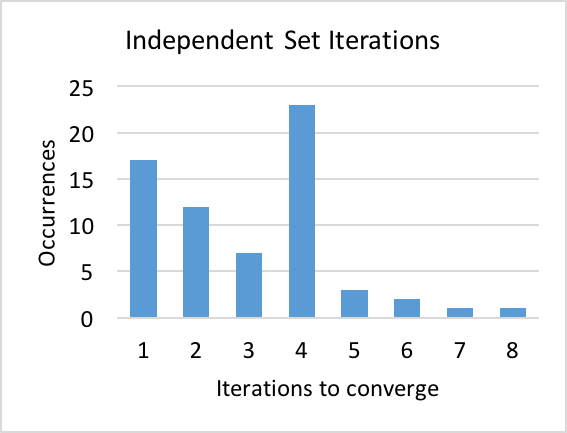
\includegraphics[width=0.5\textwidth]{indset_iters.png}}
\caption{Independent set convergence histogram}\vspace*{-6pt}
\label{fig:indset_conv}
\end{figure}

The proof of the time complexity of Luby's original algorithm
relied on probability theory and changing
the graph node numbers at each iteration \cite{luby1986simple}.
In our algorithm, the number of iterations is bounded by the
length of the longest path in the conflict graph whose nodes have monotonically
increasing quality values.
Although it may be theoretically possible to construct pathological
meshes where this path length grows proportional to the number of elements,
in practice such paths are bound by a constant.
Figure \ref{fig:indset_conv} shows a histogram of the number of
iterations required to find a maximal independent set during execution
of a typical Omega\_h mesh adaptation.
The algorithm terminates in fewer than ten iterations in all cases,
typically requiring about four iterations.

Finally, note that in line 20 of Algorithm \ref{alg:indset} we
compare graph node global IDs in the case of equal quality values.
Ties could otherwise cause the algorithm to deadlock, and we
prefer a deterministic tie-breaker.
Thus in some cases the output is affected by the global ID values,
however this does not mean it is ordering-dependent because
we update global ID values in a way that is independent
of the local ordering of entities.

\subsubsection{Ghosting for Set Selection}
\label{sec:indset_ghost}

As mentioned in Section \ref{sec:ghost}, a ghosted partition has
the useful property that every owned entity
(most importantly vertices and edges) has local copies
of all its upward adjacent entities.
All operations centered around a key entity which read information
from upward adjacent entities and write information to the
key entity can now be parallelized easily.
Every MPI rank performs the local operation around the key entities
that it owns, and then the information written to the key entities
is communicated from owned copies to all other copies.
For example, the worst element quality resulting from splitting an
edge can be evaluated locally by the MPI rank owning that edge
(because all surrounding element information is available)
and then communicated to the MPI ranks that have copies of that edge
with incomplete surrounding information.

\begin{figure}[t]\vspace*{4pt}
\centerline{
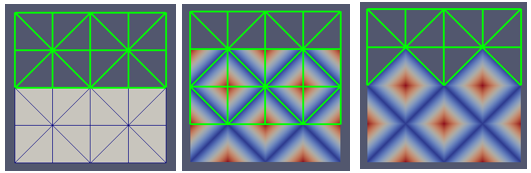
\includegraphics[width=0.7\textwidth]{mpi_indset.png}}
\caption{Steps for distributed set selection:
(left) non-ghosted partitions
(mid) add ghost layers, compute independent set
(right) trim away ghost elements not in owned independent
cavities}\vspace*{-6pt}
\label{fig:mpi_indset}
\end{figure}

During each adaptation pass in Omega\_h, we do what is possible without a ghost
layer first. Typically, this means measuring edge lengths and determining
whether any of them are too long or two short.
Then a ghost layer is constructed and possible operations are evaluated
as described in Section \ref{sec:omega_h-adapt} and
an independent set is chosen as described in Section \ref{sec:indset}.
Once an independent set has been chosen, we return to an element-based
partitioning, but one which is altered such that cavities in the independent
set reside on one MPI rank.
At that point, the code can proceed to apply the independent cavity modifications
simultaneously and produce a new local mesh structure without further communication
because entities on the partition boundary are not modified.
Figure \ref{fig:mpi_indset} illustrates this process at a simple partition boundary,
in the case of selecting which mesh vertices ought to be collapsed.

We can create the global numberings of the new mesh based on the global
numberings of the old mesh.
Entities of the same dimension are numbered together.
In an effort to preserve the spatial locality of the global numbering,
we number newly created entities based on the numbers of their old
cavity counterparts.
Specifically, we designate an entity of dimension $d$ in the old cavity
to represent all entities of dimension $d$ created in the new cavity.
If the cavity created $r$ such entities, then we assign the value
$r$ to the representative old entity.
Other $d$-dimensional entities that were destroyed by the modification
are assigned the value $0$.
Entities which stayed the same in the mesh are assigned the value $1$.
These values are put through a global exclusive scan operation
(see Section \ref{sec:scan}), resulting in offsets for the old entities.
These offsets can then be used to number the new entities.
The exclusive scan is performed in the order that entities appear
in the old numbering.
Combined with the upward adjacency sorting mechanism described
in Section \ref{sec:sort_up}, this results in a global renumbering
mechanism that is independent of partitioning and local ordering.

This overall selection process based on ghosting allows
Omega\_h mesh adaptation method to be unaffected by partition boundaries,
in the sense that the decision process of what modifications to apply
is not influenced by the partition.
The output is independent
of local ordering so long as global IDs are independent of ordering
as described above.
Most other parallel adaptation implementations that we know of explicitly
consider interior modifications first, followed by a repartitioning that
allows consideration and modification of the near-boundary mesh
\cite{loseille2015parallel,de1999parallel}, making them
at least partitioning-dependent.

\section{Determinism}
\label{sec:determinism}

Section \ref{sec:indset_ghost} described how Omega\_h takes steps
to select operations and number entities in a partitioning independent and
ordering independent way.
Omega\_h is also deterministic,
meaning that its output is the same if run twice with exactly
the same inputs, which may not be the case if it were affected
by the relative order in which distributed processes and shared
threads reach a certain point in execution.
That ordering is dependent
on computer system state beyond the control of the program,
such as other programs currently running, operating system
state, or even the physical temperature of hardware cores
altering their processing speed.

Each of these properties is important
for software development purposes for two reasons.
First, when symptoms of a bug are encountered,
it is important to be able to re-run the program with
additional instrumentation to determine the root cause.
Non-determinism can cause symptoms to appear with arbitrarily
low probability, requiring an arbitrarily large number of
trials to reproduce the issue.

If a program is partitioning-independent, a highly parallel
case that exhibits symptoms can be run with less parallelism
for debugging purposes.
As a practical example, MeshAdapt at one point had a bug
which would exhibit symptoms with sufficient probability
only using 4096 or more processes.
Much of the time required to diagnose the issue was spent
waiting for sufficient computing resources.
Conversely, if a code is partitioning-independent then
one can construct regression tests which confirm that
exactly the same results are produced with several different
partitionings.
This can catch a wide array of issues in parallel implementation.
For example, if a bug causes 0.01\% of the edge splits
along a partition boundary to be incorrectly rejected,
it may go unnoticed indefinitely for partition-dependent programs
while it would be detected by a strict comparison
of serial and parallel results.

Omega\_h is developed and debugged using a small number
of threads and processes, but has regression tests requiring
the exact same results at varying degrees of parallelism.
This tends to quickly catch parallel bugs, and it has
been scaled to thousands of GPU CUDA cores and tens of
thousands of MPI ranks without exhibiting any symptoms of
bugs that depend on the degree of parallelism.

The following sections cover two more key operations
that Omega\_h uses to establish partitioning-independence
and determinism.

\subsection{Upward Adjacency Ordering}
\label{sec:sort_up}

The mapping inversion algorithm in Section \ref{sec:invert_map}
relies on atomic operations to determine the local ordering
of upward adjacent entities, and so by itself is non-deterministic
(it depends on the temporal order in which two threads attempt to
access a single value).
We run a post-processing step which locally sorts upward adjacent
entities of a single entity by their global numbers.
Recall from Section \ref{sec:indset_ghost} that global numbers
are independent of local ordering, so this operation likewise
makes upward adjacency information independent of local
traversal order and temporal thread access order.
This is important because operations like floating-point summation
are non-associative (see Section \ref{sec:repro_sum})
and so higher-level operations like averaging values from elements
to vertices produce slightly different values depending on the
traversal order of upward adjacencies.

\subsection{Order-Independent Sums}
\label{sec:repro_sum}

Computers typically implement floating-point numbers following the IEEE 754
standard \cite{hennessy2011computer}.
This format represents real numbers as the nearest rational number
which can be represented as $(m\cdot 2^p)$, where $m$ and $p$ are both
integers within a predefined range.
Varying the exponent $p$ can be interpreted as shifting the position of the
decimal point, hence the term floating-point numbers.
The exponent $p$ is adjusted such that the digits of $m$ capture the
most significant digits of the real number being approximated.
When adding a series of floating-point numbers whose exponents
vary significantly, the resulting value can be different
depending on the order of summation.
If the values are added in descending order of magnitude, the intermediate
values will all have exponents equal to or greater than the largest
exponent $p_{\text{max}}$, so they will truncate all values less
than $2^{p_{\text{max}}}$.
When the sum follows the ascending order of magnitude, intermediate
values start with the smallest exponent and gradually increase their
exponent as small values are added.
This more accurately accumulates digits of low significance, which
may amount to a substantial difference in the final sum.

Mesh adaptation is highly sensitive to floating point values, because
as described in Chapter \ref{chap:adapt} we choose to make modifications
based on whether floating point values such as the length of an
edge in metric space are above and below an exact threshold.
Thus any perturbation could change the result of this comparison
in certain cases, and produce a different mesh topologically.
For our purposes, it is more important to have a consistent
(ordering independent) set of operations rather than the most
accurate method possible.
Simple floating point summation can be performed very quickly relative
to other mesh adaptation operations, so we prefer faster options
so long as they are consistent.
For this reason, we do not carry out a full global sort of the values
into ascending order, as that would be too expensive.
That said, we would prefer that the accuracy of our method be comparable
to that of the non-deterministic algorithm.

We add global values using a fixed-point accumulator,
meaning we select some $p_{\text{fixed}}$ and represent all
intermediate values as $M\cdot 2^{p_{\text{fixed}}}$, where $M$
is an integer.
We select $p_{\text{fixed}}=p_{\text{max}}$, which ensures that
our accuracy is at least as good as the worst-case non-deterministic
ordering, i.e. summation in descending order.
The integer $M$ must have a large enough range to store the largest
magnitude intermediate value (modulo $2^{p_{\text{fixed}}}$).
The most common format for scientific computations is a 64-bit
floating point number in which 52 bits are devoted to the integer $m$.
We devote 128 bits to our intermediate $M$ values, meaning they can
reliably add up to ($2^{76} > 10^{22}$) input values.
By comparison, the largest-scale problems being solved at the
time of this writing require summing at most $10^{12}$
floating-point values, meaning that 128 bits will remain sufficient
until the maximum problem size of interest increases
by an additional factor of $10^{10}$.
To implement this algorithm, we need to perform two reductions:
one to determine $p_{\text{max}}$, and one to add up all the
values in discrete units of $2^{p_{\text{max}}}$.
Since not all computers have built-in instructions for 128-bit
integers, we sometimes have to implement intermediate values
as a pair of 64-bit values emulating a 128-bit value.

The resulting method has a runtime that is small compared to
the other operations of mesh adaptation and produces the
exact same (bitwise consistent) values regardless of ordering.
Combining this with other techniques such as upward adjacency sorting
(see Section \ref{sec:sort_up}), we can carry out mesh adaptation
such that all floating point values are partition-independent
and ordering-independent, which is a prerequisite to having
fully independent results for the overall adaptation algorithm.

\section{Parallel Adaptation Performance}

\subsection{Generating Large Meshes}
\label{sec:big_gen}

\subsubsection{MeshAdapt Uniform Refinement}
\label{sec:ma_scale}

In order to test the capability of the hybrid MPI-thread system, PCU,
and the overall PUMI system supporting MeshAdapt,
a 1.6 billion element mesh is created using up to 16K cores of an
IBM Blue Gene/Q.

Mesh generation begins with a 4-part, 400K element tetrahedral
mesh and proceeds so as to maintain a part density of 100K elements
per part.
Each up-scaling repartitioning uses uniform mesh refinement
(see Section \ref{sec:ma_refine}), which
multiplies element counts and part counts by a factor of $8$.
At each step, we start with $2$ processes per node
and then create $8$ threads per process, repartition the mesh
among those threads with the help of migration (see Section \ref{sec:migr}),
and then apply uniform refinement using those threads.
The Blue Gene/Q has $16$ cores per node, which is why we choose $2$
processes per node so that the total threads per node equals the
number of cores per node.
At the end of each step, files are written out from each of the
threads, which will be read in by the initial processes of the
next step, where the next step allocates $8$ times more nodes
than the current step.

\begin{figure}[!ht]
\begin{center}
\caption{Times for hybrid MeshAdapt uniform refinement}
\label{fig:pcu_scale}
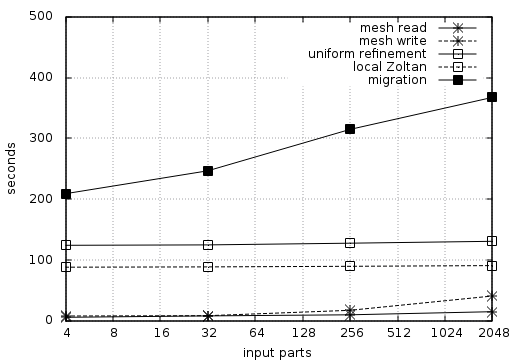
\includegraphics[width=0.7\textwidth]{pcu_scaling.png}
\end{center}
\end{figure}

Figure \ref{fig:pcu_scale} shows the time consumed by each step of the
PCU-supported MeshAdapt workflow as the number of parts is increased from 4 to
16K.
The final step converts 2K parts into 16K parts.
In this workflow, both migration and mesh file writing are being
done using 8 threads per process.
By comparison, file reading is done by the initial processes
without multi-threading,
and the times are very comparable even though each process
is writing 8 times more data, so thread parallelism is achieved
(the sizes of files are constant, so the times to read and write
a single file should be similar).
Migration shows an increase in runtime as part count is
increased, which can be correlated with Figure \ref{fig:neighbor}, which
shows how the number of neighbors of a mesh partition
are increasing at the same rate as the migration runtime,
both of which grow logarithmically with the number of elements and partitions.
Recall that the exchange algorithm described in Section \ref{sec:exch}
and migration in general have runtimes proportional to the number
of neighbors.

\begin{figure}[!ht]
\begin{center}
\caption{Neighborhood increase during MeshAdapt uniform refinement}
\label{fig:neighbor}
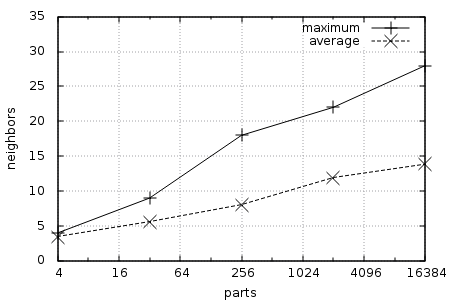
\includegraphics[width=0.6\textwidth]{pcu_neighbor.png}
\end{center}
\end{figure}

After generating this mesh, we study the overhead of threading with
a simple workflow.
Beginning with $P$ processes and $T$ threads per process
such that $(P\cdot T)$ always equals 16K, we read the 16K-part,
1.6 billion element mesh.
In terms of hardware, we are using 16K cores of the Blue Gene/Q,
which is 1024 nodes or one full rack.
Then every thread migrates 10K elements to one of its
neighbors.
The resulting mesh is then written out.
All operations are done in the hybrid mode, and the
number of threads per process $T$ is varied.
In all cases, the ideal outcome is that runtime
remains the same.

\begin{figure}[!ht]
\begin{center}
\caption{Hybrid File IO performance}
\label{fig:pcu_fileio}
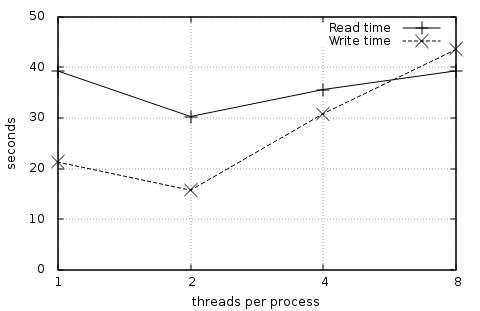
\includegraphics[width=0.6\textwidth]{pcu_fileio.png}
\end{center}
\end{figure}

Figure \ref{fig:pcu_fileio} shows the times for hybrid file IO.
File IO is more prone to fluctuation because the filesystem
and associated networks are shared by all users of the supercomputer.
Despite this, we see file IO performance remains
fairly constant as we move from process-only to hybrid operation.

\begin{figure}[!ht]
\begin{center}
\caption{Hybrid migration performance}
\label{fig:pcu_migrate}
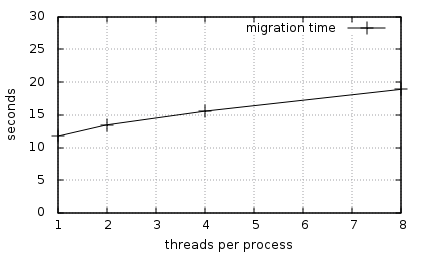
\includegraphics[width=0.6\textwidth]{pcu_migrate.png}
\end{center}
\end{figure}

Figure \ref{fig:pcu_migrate} shows migration time over threads per process.
Since the ideal result is constant, we see a logarithmic overhead
in this part of the workflow.

\subsubsection{Omega\_h Parallel Size Field Scaling}
\label{sec:osh_scale}

In order to carry out a study similar to the one in Section \ref{sec:ma_scale}
using Omega\_h instead of MeshAdapt, we choose to use general mesh
adaptation with a scaled size field because Omega\_h does not use refinement
templates, including the uniform refinement template.
We therefore parallelize the size field scaling workflow from
Section \ref{sec:scale_test}.
Our initial geometry, as illustrated by Figure \ref{fig:osh_scale}, is
a $4\times 4$ array of the solder ball geometry used in Section \ref{sec:scale_test}.
The initial mesh contains 80K elements.
At each step $i$, two programs are run.
The first program uses $P=2^i$ processes to read a mesh of $2^{i-1}$
parts and use global Recursive Inertial Bisection to repartition it
into $2^i$ parts \cite{simon1991partitioning}.
The second program uses $P=2^i$ processes to compute the implied
isotropic size field, scale it with the goal of obtaining
$(80\cdot 10^3 \cdot 2^i)$ elements, and run mesh adaptation.
At all times we use $\lceil 2^i / 16 \rceil$ nodes such that there are
at most $16$ processes in a node.
Note that because we use size field scaling, we can multiply
by a factor of $2$ at each step, whereas uniform refinement
is limited to a factor of exactly $8$, which can be too coarse
a mechanism for achieving a desired element count.

\begin{figure}[t]\vspace*{4pt}
\centerline{
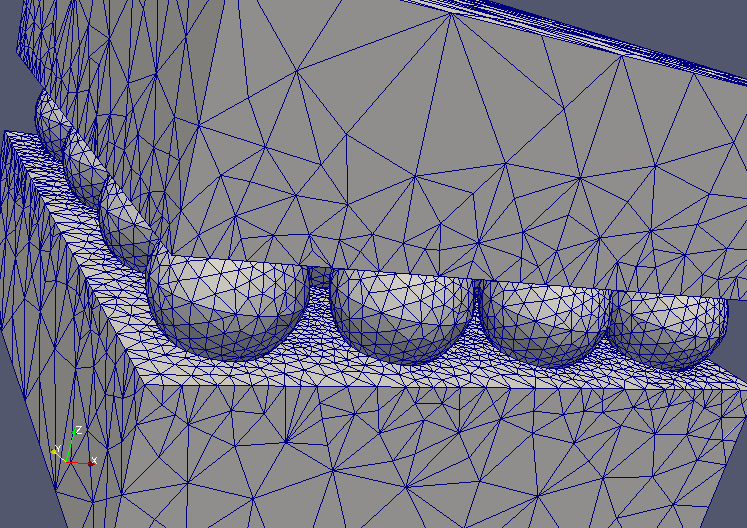
\includegraphics[width=0.45\textwidth]{sb_160k.png}
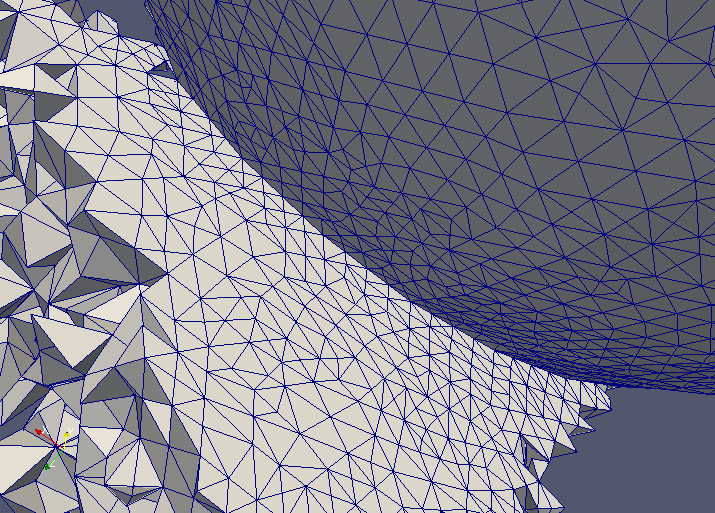
\includegraphics[width=0.45\textwidth]{sb_20480k_part40.png}
}
\caption{(left) the $4\times 4$ solder ball mesh with 160K elements,
(right) one of 256 partitions of the mesh with 20M elements}
\label{fig:osh_scale}
\end{figure}

Table \ref{tab:osh_scale} shows several performance metrics collected
during this study.
The correlation between actual and target element counts is consistent
with the behavior described in Section \ref{sec:scale_test}.
Both repartitioning and adaptation times show good scalability,
growing roughly logarithmically with the number of elements and parts,
with the notable exception of the jump in repartitioning time
to reach 8K parts.
Note that here we are exercising all components
of adaptation described in Section \ref{sec:omega_h-adapt}, not just
refinement.
Even collapses are exercised, as the edge length loop in
Section \ref{sec:osh} will carry out many collapses of short
edges created during refinement (e.g. splitting the long edge
of an obtuse triangle creates a very short edge).
These components are all parallelized using the methods described
in Sections \ref{sec:indset}, \ref{sec:indset_select}, and
\ref{sec:indset_ghost}, and all of them scale well in this study.
Memory usage per part shows a similar pattern of scalability.
The speedup in the last column is the weak scaling speedup,
computed as the number of processes times the parallel
efficiency, where parallel efficiency is the slowdown
in adaptation compared to ideal linear scaling.

\begin{table}
\caption{Performance metrics of Omega\_h parallel scaling}
\label{tab:osh_scale}
\begin{center}
\begin{tabular}{r|r|r|r|r|r|r}
target & actual & repart. & adapt &
MB  & parts & speedup \\
elements & elements & time & time &
per & & \\
$(\times 10^3)$ & $(\times 10^3)$ & (sec.) & (sec.) &
part & & \\\hline
     160 &     160 & 4.52 & 398 & 149 &     2 &    2 \\
     320 &     283 & 6.46 & 362 & 125 &     4 &    4 \\
     640 &     566 & 6.26 & 409 & 133 &     8 &    8 \\
    1280 &    1146 & 6.18 & 370 & 119 &    16 &   17 \\
    2560 &    2340 & 8.13 & 385 & 117 &    32 &   33 \\
    5120 &    4615 & 8.78 & 482 & 131 &    64 &   53 \\
   10240 &    9320 & 10.5 & 422 & 110 &   128 &  121 \\
   20480 &   18784 & 10.8 & 525 & 129 &   256 &  194 \\
   40960 &   37273 & 16.8 & 544 & 138 &   512 &  374 \\
   81920 &   74847 & 22.1 & 607 & 148 &  1024 &  671 \\
  163840 &  150338 & 34.1 & 660 & 157 &  2048 & 1235 \\
  327680 &  299090 & 46.8 & 677 & 159 &  4096 & 2408 \\
  655360 &  599510 &  165 & 711 & 160 &  8192 & 4586 \\
 1310720 & 1201815 &  146 & 876 & 190 & 16384 & 7444 \\
\end{tabular}
\end{center}
\end{table}

\subsection{Non-Uniform Size Field with Load Balancing}

The test in Section \ref{sec:osh_scale} demonstrates the scalability of
adapting to a uniform size field.
However, many interesting load balancing and performance considerations
come into play when adapting to a non-uniform size field,
and this section studies that capability using Omega\_h.
First, recall from Section \ref{sec:elem_count} that in the process
of targeting a particular element count we derived a formula to predict
how many output elements an input element would generate during adaptivity,
based roughly on its size in metric space.
We can use these values as weights in a load-balancing problem, such that
partitions are created not only on how many elements they have prior to
adaptation, but also based on how many they will have at the end of adaptation.
If a partition is sized based on input elements and it ends up refining
much more than others, then during or after adaptation a load imbalance and
possibly a memory overflow (of the memory space where this partition is)
could occur.
Conversely, if a partition is sized based only on output elements, and it
is due for heavy coarsening, then before adaptation we again have severe
imbalance and possibly a memory overflow.
Thus, our load-balancing weight for an element is actually the average of $1.0$
and the predicted output element count of the given element,
where $1.0$ represents how many elements the element is prior to adaptation.
In this way we establish a partition which is halfway between the optimal
partitions for input and output meshes.

The above load balancing algorithm is here referred to as predictive
load balancing.
After adaptation, we apply a post-processing load balance step based
on the exact number of output elements.
Figure \ref{fig:tall} illustrates this process on a geometry that is
purposely elongated to induce a 1D partitioning when our Recursive
Inertial Bisection method is used.
The initial mesh is uniformly sized, and the first part of
Figure \ref{fig:tall} shows the desired size field, which is three
times larger at the top and bottom than at the center.
The following four parts of Figure \ref{fig:tall} show how the mesh
is initially partitioned, how the predictive load balancing increases
the size of the top and bottom partitions to account for their coarsening
(but only halfway), and how after adaptation the other half of the distance
is covered by post-balancing to arrive at a well-balanced partitioning.
In this example, the mesh is perfectly balanced at the start and end
of the workflow (to within $\pm 1$ element), and the ``halfway" partition
used for adaptivity has an imbalance value of $1.32$, where imbalance
is defined as the maximum partition size divided by the average partition size.

\begin{figure}
\begin{center}
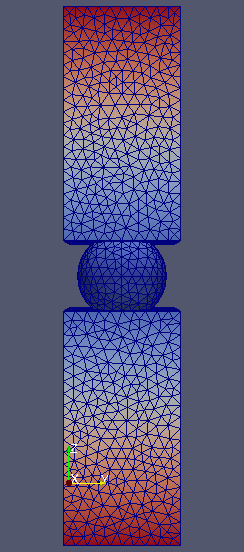
\includegraphics[width=0.18\textwidth]{tall_size.png}
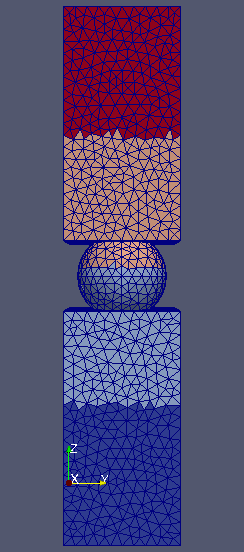
\includegraphics[width=0.18\textwidth]{tall_input.png}
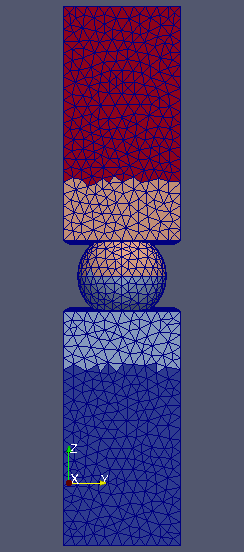
\includegraphics[width=0.18\textwidth]{tall_predictive.png}
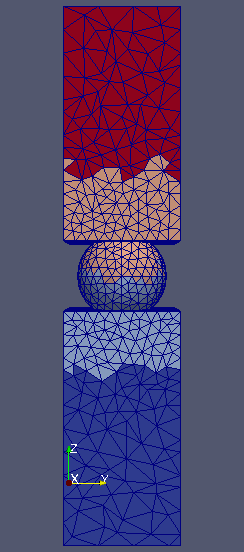
\includegraphics[width=0.18\textwidth]{tall_adapted.png}
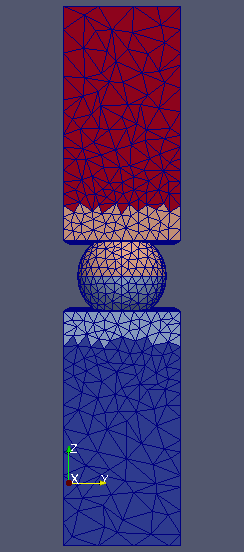
\includegraphics[width=0.18\textwidth]{tall_post.png}
\caption{Left to right: size field, input partitions, predictive partitions,
adapted partitions, and post-balanced partitions
for a simple 4-part problem}
\label{fig:tall}
\end{center}
\end{figure}

We now take this same non-uniform size field in which the center of a solder
ball geometry aims to be 3X finer than the top and bottom, and conduct
a scaling study on an IBM Blue Gene/Q computer.
We start with a uniformly-sized 90 million element mesh, which is
partitioned into versions with 2048, 4096, and 8192 parts.
A 195K element version of this mesh is shown in Figure \ref{fig:slope_195k}.
Then each version is adapted to the non-uniform size field using
the predictive method described above.
We use size field scaling to ensure the mesh has about 90 million
elements after adaptation, and in all cases we do end up
with 89.5 million elements (recall that Omega\_h produces the
same mesh regardless of partitioning).
Since the size of the problem is constant (i.e. we are ``strong scaling"),
we expect runtime to decrease in proportion to the increase
in parallelism.
Table \ref{tab:slope_scale} shows the adaptation times,
speedups relative to the 2048 part case, and imbalances
after ``halfway" predictive load balancing and after
adaptation.
Before predictive load balancing and after post-balancing,
there is essentially no imbalance ($1.0\pm 10^{-4}$).
Since the goal of our predictive method is to find the middle
ground between partitions optimal for the input and output
meshes, then we expect that if we are successful the
imbalance values after predictive balance and after
adaptation will be similar, i.e. two values which
vary inversely to one another are minimized by making
them equal.
We do see these two imbalances being close in
Table \ref{tab:slope_scale}.

\begin{figure}
\begin{center}
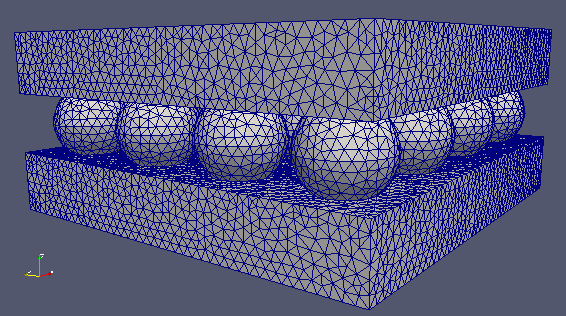
\includegraphics[width=0.6\textwidth]{uniform_195k.png}
\caption{A 195K element version of the 90M element mesh
used for the non-uniform size field strong scaling study}
\label{fig:slope_195k}
\end{center}
\end{figure}

\begin{table}
\caption{Strong scaling with non-uniform size field}
\label{tab:slope_scale}\vspace*{4pt}
\centerline{
\begin{tabular}{r|r|r|r|r}
\#parts & predictive & adapted   & adapt   & speedup \\
        & imbalance  & imbalance & time    & \\
        & (max/avg)  & (max/avg) & (seconds) & \\\hline
   2048 &      1.658 &     1.797 & 1447    & 1.00  \\
   4096 &      1.722 &     1.874 &  828    & 1.74 \\
   8192 &      1.775 &     1.941 &  507    & 2.85 \\
\end{tabular}
}
\end{table}

\subsection{Moving Objects on Shared Memory Devices}

In this test case, we focus on the potential for mesh adaptation to support simulations
that have 3D solid bodies moving through a fluid.
Mesh adaptation can be used to adjust connectivity between iterations of
mesh motion, preventing tangling and inversion.
Several other researchers have made good progress in applying general adaptation
for these purposes
\cite{compere2010mesh,wicke2010dynamic,clausen2013simulating,chen2015parallel}.
In this test case, we created a geometry consisting of two ``rotors" whose ranges of
motion overlap.
This geometry is meant to be similar to simulations of interest such as
helicopter rotors and manufacturing processes in which a fluid product is
stirred.

\begin{figure}[t]\vspace*{4pt}
\centerline{
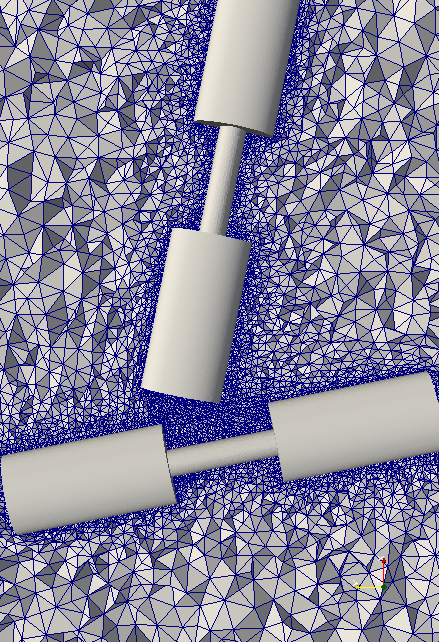
\includegraphics[width=0.3\textwidth]{twin_rotor_1.png}
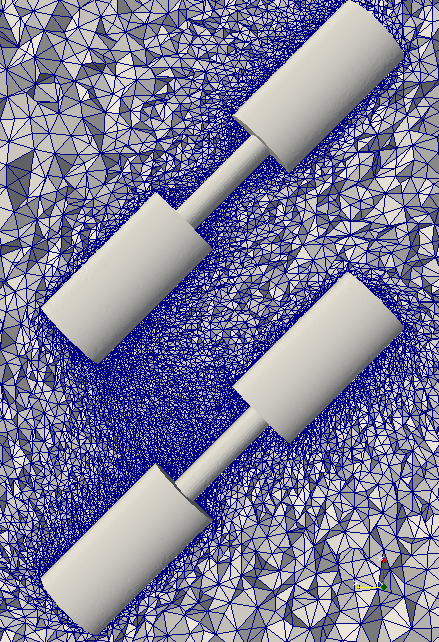
\includegraphics[width=0.3\textwidth]{twin_rotor_2.png}
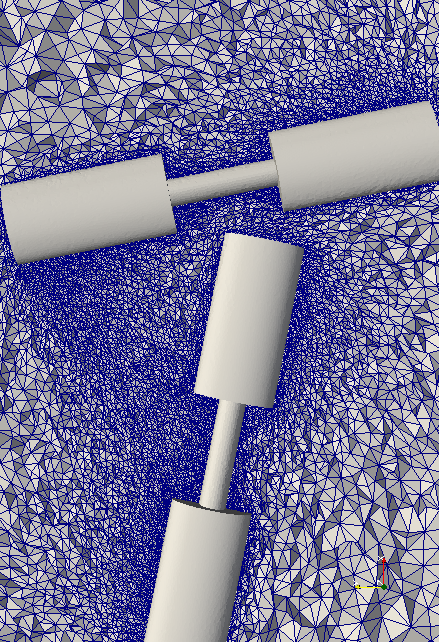
\includegraphics[width=0.3\textwidth]{twin_rotor_3.png}
}
\caption{Cutaway mesh views at steps 2, 8, and 14 of 16}\vspace*{-6pt}
\label{fig:twin_rotor}
\end{figure}

\begin{table}
\caption{Runtime in minutes on different hardware}
\label{tab:twin_rotor_times}\vspace*{4pt}
\centerline{
\begin{tabular}{l|r|r|r|r|r| r| r| r}
 & \multicolumn{7}{c}{number of OpenMP threads} \\
Hardware              & GPU &    1 &   2 &   4 &   8 & 16 & 32 & 64 \\\hline
Intel Xeon 2620 v4    &     &  203 & 115 &  76 &  55 &    &    &    \\
Intel Knights Landing &     & 1196 & 598 & 299 & 153 & 79 & 42 & 24 \\
NVidia K80            &  35 &      &     &     &     &    &    &    \\
NVidia GTX 980 Ti     &  15 &      &     &     &     &    &    &    \\
\end{tabular}
}
\end{table}

The case is executed in a series of 16 time steps, where the
following happens at each step:
\begin{enumerate}
\item A velocity field is prescribed for each object as vectors
at mesh nodes.
\item This velocity field is spread onto the surrounding fluid
mesh nodes by solving Laplace's equation using the
objects and domain boundary as Dirichlet conditions.
\item The mesh is moved according to the velocity field
and stops right before any element goes below 20\% mean ratio quality.
Using a lower threshold here causes quality repair to take much longer
or fail.
\item Mesh adaptation is applied to the deformed mesh to
recover edge lengths and ensure all elements are above 30\%
mean ratio quality.
Our shape correction algorithms can have difficulties bringing
all elements above a higher threshold than this.
Mesh adaptation will rebuild the mesh about ten times when applied.
\item Steps 2 to 4 are repeated for any remaining motion
that would previously have inverted elements.
This repetition occurs ten to twenty times per time step.
\end{enumerate}
We generated the initial mesh
using Gmsh \cite{geuzaine2009gmsh} with optimization by Netgen
to remove sliver elements.
All subsequent motion and adaptation is handled by our code.
Figure \ref{fig:twin_rotor} shows cutaway views of the mesh
after time steps 2, 8, and 14 out of 16.
The number of elements increases from one million to two
million from start to finish.

Table \ref{tab:twin_rotor_times} shows the runtime performance across
different hardware.
We first run on an Intel Xeon processor typical of current servers
and clusters.
Then, we run the same case on two pieces of hardware found on
current supercomputers: the Intel Knights Landing CPU
and the NVidia Tesla K80 GPU.
Finally, we also run on a more consumer-market GPU,
the NVidia GTX 980 Ti.
Unlike CPUs, GPUs do not offer clear controls for using a subset
of threads, so it is typical to simply show GPU speedup versus
serial (in this case, 7X for the GTX 980 Ti) as opposed to some
kind of scaling on the GPU.
The Xeon 2620 has 8 cores and the Knights Landing CPU has
64 cores, and we see decent scaling until the number
of OpenMP threads equals the number of cores, on both CPUs.

%%% Local Variables:
%%% mode: latex
%%% TeX-master: t
%%% End:

